This chapter builds upon the insights collected in the previous chapters. Based on these findings, this study shall undertake empirical research. The concepts and techniques used to undertake the empirical research shall be discussed here. 
\section{Research design}
This study aims to investigate the long term relationship between the B-BBEE policy and firm performance. Based on, among other sources, the findings from the Contextualization and Theory chapter, this section operationalizes long term, B-BBEE policy and firm performance. The empirical research aims to follow a deductive approach, whereby the observable data and literature makes room for testing the hypothesis [61]. The empirical research moves from general frame of observations to the specific answer.  
\subsection{Research questions}
The main research question posed in the Introduction chapter is: \textbf{“What is the long term relationship between the Broad-Based Black Economic Empowerment policy on firm profitability of Johannesburg Stock Exchange-listed companies?”}.

To answer this research question several sub questions arise. The long term impact can be for example tested over the entire time period from 2004 to 2018. This creates the research subquestion: \textbf{“What was the long term relationship between Broad-Based Black Economic Empowerment policy on firm profitability of the Johannesburg Stock Exchange-listed companies over the period 2004 - 2018?”}. As discussed in the Contextualization chapter, the Codes of good practise changed, therefore B-BBEE could be subdivided into the periods 2004 - 2007, 2007 - 2013, and 2013 to 2018. This study poses the sub research questions: \textbf{What was the long term relationship between B-BBEE policy and firm performance among the three B-BBEE policy periods?”}. Finally, as the Theory chapter, section compliance effects indicates, some industries would have a higher incentive to comply to B-BBEE policy. Therefore the sub question arises: \textbf{“Did firms operating in a sector with a higher incentive to comply to the B-BBEE policy have higher firm performance?”}.
\subsection{Hypothesis}
Hypotheses provide a clear falsifiable statement upon which support to answer the research question. The hypotheses are based upon findings from previous research [4 ,p44].

In terms of BEE/B-BBEE, recall that the objective of the policy was to reduce wealth inequality, which requires commitment from firms. This study argues that a positive relationship between B-BBEE and firm performance should exist to incentivize firms to empower Black people. The null hypothesis there is:
\begin{nullhypothesis}The long term relationship between B-BBEE rank and share price return of Johannesburg Stock Exchange-listed companies is positive\end{nullhypothesis}
the alternative hypothesis is:
\begin{alternativehypothesis}The long term relationship between B-BBEE rank and share price return of Johannesburg Stock Exchange-listed companies is not positive\end{alternativehypothesis}
These hypotheses will be tested through statistical analysis. If there is statistical evidence then the alternative hypothesis will be accepted and the null hypothesis will be rejected. The hypothesis is tested using a non-directional, two tailed t-test, similar to Mokgobinyane [4, p45]. Rejection of the null hypothesis indicates that the policy measure has failed over the long term. A positive relationship implicates that a high B-BBEE rank causes a high share price return. Vice versa, a negative relationship implies that a high (low) B-BBEE rank causes a low (high) share price return.
\section{Research method}
This study quantitatively test the hypotheses using an ordinary least squares regression analysis. Most of the prior research on the long term relationship between B-BBEE aggregate score and share price return have deployed ordinary least squares regression analysis and no indication was presented of non-linearity of the findings. There are 2 models tested. Model 1, the FF model, resembles the Fama and French model:
\begin{equation}
\begin{aligned} %https://tex.stackexchange.com/questions/194236/why-does-not-go-to-new-line-in-equation - makes sure equation stays in marging of page
    R_{it} = R_{ft} + \beta BBBEE_{it} + \beta BBBEE_{iM}[E(R_{Mt}) - R_{ft}] \\
    + \beta_{iBP} BP_t + \beta_{iSIZE} SIZE_t +  \beta IND_{it} + \epsilon_{it}
\end{aligned}
\end{equation}
where $R_{it}$ is the share price return of observation $i$ at time $t$, $R_{ft}$ is the risk free return at time $t$, $\beta BBBEE_{it}$ is the B-BBEE rank for observation $i$ at time $t$, $\beta BBBEE_{iM}[E(R_{Mt}) - R_{ft}]$ is the (beta) coefficient of observation $i$ for the market risk premium at time $t$ over the risk free return at time $t$, $\beta_{iBP} BP_t$ is the (beta) coefficient of observation $i$  for index of high minus low book to market value at time $t$, $\beta_{iSIZE} SIZE_t$ is the (beta) coefficient of observation $i$  for the index of high minus low market capitalization at time $t$, $\beta IND_{it}$ are the coefficients of observation $i$ for the vector of industry dummy variables at time $t$ and $\epsilon_{it}$ is the error term for observation $i$ at time $t$. 

Model 2, the MF model is defined similarly to the model defined by Merwe and Ferreira:
\begin{equation}
\begin{aligned} %https://tex.stackexchange.com/questions/194236/why-does-not-go-to-new-line-in-equation - makes sure equation stays in marging of page
    R_{it} = \alpha_0 + \beta BBBEE_{it} + \beta BP_{it} + \beta SIZE_{it}     + \beta EP_{it} + \beta IND_{it} + \epsilon_{it}
\end{aligned}
\end{equation}
where $R_{it}$ is the share price return of observation $i$ at time $t$, $\alpho_0$ is the constant, $\beta BBBEE_{it}$ is the B-BBEE rank  for observation $i$ at time $t$, $\beta BP_{it}$ is the (beta) coefficient of observation $i$ of book to market value of observation $i$ at time $t$, $\beta SIZE_{it}$ is the (beta) coefficient of observation $i$ to market capitalization of observation $i$ at time $t$, $\beta EP_{it}$ is the (beta) coefficient of observation $i$ to the earnings to price ratio of observation $i$ at time $t$, $\beta IND_{it}$ are the coefficients of observation $i$ for the vector of industry dummy variables at time $t$ and $\epsilon_{it}$ is the error term for observation $i$ at time $t$. This model closely follows the methodology of van der Merwe and Ferreira. 

Testing both the Fama and French model and Merwe and Ferreira model adds to the robustness of the empirical analysis. Model 1, based upon the Fama and French model could yield more observations. As only the beta coefficient to the index is required, more observations can be included. In model 2, based upon the van der Merwe and Ferreira model the book to market of a firm at a particular time is used. However, when the book to market of a firm is unavailable, then this firm at this particular time is discarded. On the other hand,  replicating the model of van der Merwe and Ferreira offers comparability.

Apart from the two models, a bootstrap simulation is ran to investigate whether compliance to the B-BBEE policy in a particular industry resulted in higher firm performance, to answer the research sub question posed in the section “Research questions”. The advantage of running a bootstrap simulation is that this simulation does not require Gaussian assumptions. This adds to robustness of this study’s empirical analysis. To run the bootstrap simulation, B-BBEE observations are randomly resampled in a particular year. Then, the mean is calculated. This resampling is done 10,000 times for this particular year, resulting in a top 95\% mean and bottom 5\% of the generated means. This exercise is repeated for each of the years. These confidence intervals are not subject to normal distribution assumptions. The average performance of the top and bottom 30\% B-BBEE compliant firms for each year is then compared against the confidence intervals. A significant positive relationship is established when the top or bottom 30\% B-BBEE outperforms the top 95\%. This method resembles the bootstrap methodology used by Mehta and Ward. The selection for 30\% as the cut of for top and bottom B-BBEE was inspired by the cut off Fama and French used for the calculation of the Fama and French factors.
\subsection{Replicability}
The models, and their accompanied results were coded using Python. The repository with code is available through github \url{https://github.com/OmegalGangapersad/MasterThesis}. This study argues that composing models in an universally popular open source coding language such as Python and making this code available through github increases the transparency and replicability of this study.
\subsection{Defining long term}
The body of research discussed in the section “Previous research on the relationship between B-BBEE scores and firm performance” uses a time horizon of one year to investigate the long term effect of B-BBEE on firm performance. Merwe and Ferreira note that using a time horizon of one year is not sufficient to capture the efficacy of the policy. [7, p554]. This research adds to the body of research by investigating the relationship between B-BBEE score and share price return, one, two, three, four and five years forward. The long history of B-BBEE enables this research to perform these analyses. 
\section{Variables and data collection}
This section defines the variables mentioned in the research method and provides justification for selecting these variables. Finally this section will disclose how the the data on these variables were collected.  
\subsection{Dependent variable - firm performance}
This thesis aims to investigate the influence of B-BBEE scores on firm performance. In terms of BEE, recall that the objective of the policy was to reduce wealth inequality. In order to reduce wealth inequality, in the long term, the firm’s operation must be sustainable. Put straightforward, a firm can score high on all scores except for shareholder return, and therefore address wealth inequality. However, if the firm only destroys shareholder return, this firm will cease to exist when the firm can no longer find means to finance itself. Should B-BBEE therefore create a sustainable wealth inequality reduction, then in the long term profitability should increase or at minimum not decrease. Profitability therefore still presents a suited indicator of firm performance to test whether the B-BBEE policy was effective. Firm performance measurements are ambiguous. The research discussed in the Theory used measurements of profitability. Mokgobinyane for example used, Revenue, Net profit margin and return on equity [4, p48; 4, p49]. Other studies such as Merwe and Ferreira used share price return. 

This study argues that share price return is the best suited measurement for firm performance. Companies with higher profitability have been observed to attract more investment flows which drive share price performance [4, p59]. Investment flows can be viewed as, a reflection not of current profitability of the firm, but projected future profitability of the firm. This relates to the long term prospects that are incorporated in share price returns. Further, conventional investment decisions typically are based on discounted future cash flows. The forward looking character of investment flows should allow it to smoothen capital expenditures, such as B-BBEE related costs. Capital expenditures however could have ad hoc impact on backward looking profitability measures such as net profit margin and return on equity. Investment flows also impact the cost of funding of a firm. For example, according to research, credit ratings are lower for firms that have superior sustainability scores lowering the cost of debt [16, p24]. Credit ratings are obtained by independent credit agencies that examine the creditworthiness of a firm, the better the credit rating the lower interest rate a firm has to pay. Within the broader ESG research field, it is argued that good employee relations lower uncertainty and therefore lowers the cost of equity [16, p25]. These dynamics are not captured by for example revenue growth. Argued from an alternative vantage point, institutional investors such as pension funds are increasingly obliged by regulators and governments to incorporate ESG score into their investment decision-making process, will drive up share price. Within the realm of this study, the South African sovereign wealth fund Public Investment Corporation, must invest in B-BBEE compliant firms [23, p27]. This increases the share price of B-BBEE compliant firms strengthens the firm. A firm could for example leverage the share price inflation to raise money from the public equity markets which would allow the firm to achieve economies scale of advantages. Finally, measures such as return on equity and net profit margin can be manipulated through accounting tricks or decisions by management. For example, a company can generate a higher net profit margin by delaying expenses. Share price return of large firms, however, is not as easily manipulated.

The unit that will be analyzed is the dependent variable share price return defined as a daily return calculated as natural log return. The returns are calculated from August to August, as proposed by Merwe and Ferreira. Considering that the B-BBEE score (mentioned in the next paragraph) is released in April, that the lag allowed for the market to incorporate the information of B-BBEE scores is 4 months. This data is obtained through Thomson Reuters Datastream. As discussed in the section time horizon over which this return is calculated is one, two, three, four and five years.
\subsection{The treatment variable - B-BBEE policy}
The B-BBEE policy is measured through adherence to the goal of the policy, empowering Black people. This adherence is measured by ranking firms on their B-BBEE aggregate score each year. The source of this data from 2016 to 2018 was retrieved directly from Empowerdex through the website of their holding company, Intellidex. Colin Anthony, GM of Intellidex Investment Media, provided B-BBEE scores 2011 to 2015.  Finally, van der Merwe supplied B-BBEE scores in excel from 2005 to 2011. The source of van der Merwe was also from Empowerdex, therefore the creator of the scores was consistent, namely Empowerdex.

As visualized in the below figure, the availability of BBBEE rank varied significantly by year.
\begin{figure}[!h]
  \centering
  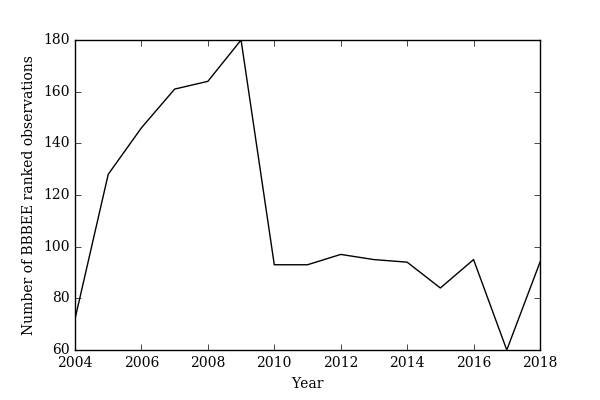
\includegraphics [scale=0.5]{ScatterPlot_Year_BBBEE_Rank.png} \\
  {\small {\it \caption{Available B-BBEE rank observations per year\label{fig:moun}}}}
\end{figure}

The BBBEE ranks were retrieved through the Empowerdex top 100 JSE Most Empowered Companies, as mentioned in the methodology. Interestingly, it appears that the Empowerdex top 100 in pre 2010 mostly exceeded 100 firms. From 2010 onwards, the number of observations with a BBBEE rank dropped to below 100 firms. The reason why the BBBEE rank dropped below 100 firm, instead of equal to 100 firm as one would expect from a top 100, is that firms for which no price was available (price was retrieved from Thomson Reuters Datastream) were excluded. This resulted in an average of 5 firms being excluded, therefore an average of 95 firms available each year. Notably, in 2017 the number of firms dropped to 62. The BBBEE rank for 2017 were retrieved from the Intellidex website. It appears that the amended codes were made obligatory by 2017, yielding in the drop of observations in 2017. The variability of observations required adjustments to prevent outcomes biased to the pre 2010 period. Put straightforward, as most observations were from pre 2010 this analysis would be moreso a reflection of the pre 2010 period, rather than the entire 2004 - 2018 period. Therefore, the number of BBBEE rank was capped at 60, to create a uniform distribution of observations through time.
\subsection{Control variables}
The risk free rate is defined as the yield on the 10 years South African Government bond. The yields of the 10 years South African Government bond is obtained through Thomson Reuters Datastream. The value factor is the book value per share as stated in Thomson Reuters Datastream. The book value per share equals the book market to market capitalization ratio. The size factor is the market capitalization factor and obtained through Thomson Reuters Datastream. The earnings to price ratio equals the earnings yield, which is defined as the earnings divided by the closing price of a firm. This ratio is retrieved from Thomson Reuters Datastream.

The Fama and French model uses three indices; market risk premium, BP Index and SIZE index. The constituents of these indices at any point in time depend on the universe of firms at that particular time. The availability of these firms depends on the availability of B-BBEE rank. Put straightforward, the  market risk premium is calculated as the average return of the firms available each year. The firms available each year depends on the availability of B-BBEE rank.  The BP Index follows the Fama and French methodology, therefore the return of the BP Index equals the average return of the 30\% highest book to market ratio firms at a particular time minus the average return of the 30\% lowest book to market ratio firms at a particular time. The number of firms in total available, to emphasize, depends on the availability of B-BBEE rank. At the different time frames (one, two, three, four, five years) these indices represent the return of these indices over the different time frames, therefore the BP Index on a two years time frame represents the average two year return of the 30\% highest book to market ratio firms at a particular time minus the average return of the 30\% lowest book to market ratio firms at a particular time.

Instead of using industry categorization through the Codes of good practise, this study based industry classification based on the ICB Industry name, which is gathered through the Thomson Reuters Datastream Industry Level 2 Sector Name. Using the industry classification from Thomson Reuters Datastream prevents the industry classification inconsistencies encountered in the Mokgobinyane study.